\documentclass{article}

\usepackage{fontspec}
\setmainfont{Liberation Serif}

\newcommand{\autor}{Jakson Alves de Aquino}
\newcommand{\titulo}{Communication between Neovim and R}

\title{\titulo}
\author{\autor}
\date{\today}

\usepackage{tikz}

\definecolor{darkgreen}{rgb}{0.0, 0.8, 0.0}

\begin{document}

\thispagestyle{empty}

\begin{center}
    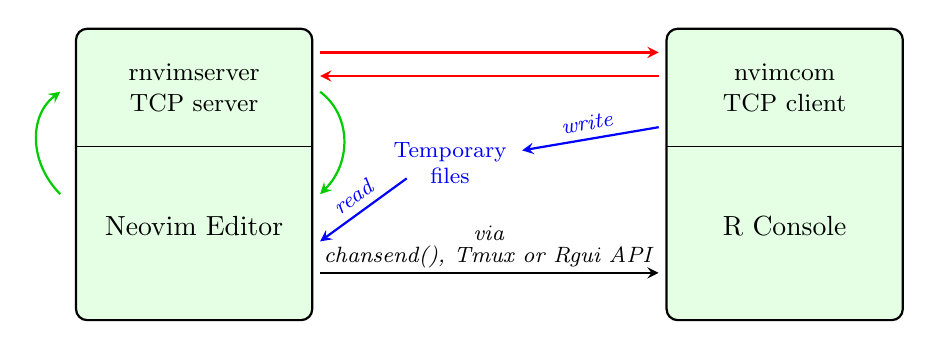
\begin{tikzpicture}[scale=1.0, >=stealth, node distance=1cm]
        \normalsize
        \draw [thick, fill=white!90!green, rounded corners] (7.5, 2.8) rectangle (10.5, 6.5);
        \draw [thick, fill=white!90!green, rounded corners] (0, 2.8) rectangle (3, 6.5);
        \node (vimed) at (1.5, 4) {Neovim Editor};
        \node (rcon) at (9, 4) {R Console};
        \small
        \draw (0, 5) -- (3, 5);
        \node (pysrv) at (1.5, 5.75) [text width=2cm, align=center] {rnvimserver TCP server};

        \draw (7.5, 5) -- (10.5, 5);
        \node (vcsrv) at (9, 5.75) [text width=2cm, align=center] {nvimcom TCP client};

        \footnotesize
        \draw [->, thick] (3.1, 3.4) -- (7.4, 3.4);
        \node at (5.25, 3.9) {\emph{via}};
        \node at (5.25, 3.6) {\emph{chansend(), Tmux or Rgui API}};

        \node [shape=circle, text width=1.5cm, align=center, blue] (tmpf) at (4.75, 4.80) {Temporary files};
        \draw [<-, thick, red] (7.4, 6.20) -- (3.1, 6.20);
        \draw [->, thick, red] (7.4, 5.90) -- (3.1, 5.90);
        \draw [->, thick, darkgreen] (3.1, 5.70) .. controls (3.5, 5.40) and (3.5, 4.80) .. (3.1, 4.40);
        \draw [<-, thick, darkgreen] (-0.2, 5.70) .. controls (-0.60, 5.40) and (-0.60, 4.80) .. (-0.2, 4.40);
        \draw [->, thick, blue] (7.4, 5.25) -- (tmpf) node[above, sloped, midway] {\emph{write}};
        \draw [->, thick, blue] (4.2, 4.6) -- (3.1, 3.8) node[above, sloped, midway] {\emph{read}};
        \normalsize
    \end{tikzpicture}
\end{center}


\end{document}
